\section{Testing and documenting the system}

\phantomsection

Software Testing is necessary because we all make mistakes. Some of those mistakes are unimportant, but some of them are expensive or dangerous.   We need to check everything and anything we produce because things can always go wrong – humans make mistakes all the time.  There is nothing better than a strongly tested software.  Imagine that you spent a lot of time developing something that is not gone used by real users because it’s buggy.  Since we assume that our work may have mistakes, hence we all need to check our own work.\vspace{0.3cm}

However some mistakes come from bad assumptions, so we might make the same mistakes when we check our own work as we made when we did it. So we may not notice the flaws in what we have done. One of the most important things to do if you want to have a successful release and to promote an application and make it popular is to permanently monitor the crash rate of the application and keep it as small as it’s possible.  Because nobody likes when the application is crashing or when something is not working as it’s supposed.But how to keep the crash rate of an application small? Ideally, we should get someone else to check our work because another person is more likely to spot the flaws. \cite{unit-test} \vspace{0.3cm}

But usually, in startups, there is not enough money to pay for human resource and to have quality engineers that will test the application manually and will assure it’s quality. That’s why a good solution would be to have a crash-free application by writing unit tests, instrumentation tests, snapshot tests which were done for the system and will be described below.\vspace{0.3cm}

\textbf{Application's views}

In this section it will be explained how the application works and what the user is able to do with this application. It will be explained all the use cases, starting from camera listing to time-lapse management.

\vspace{0.3cm}
\begin{figure}[!ht]
   \centering
   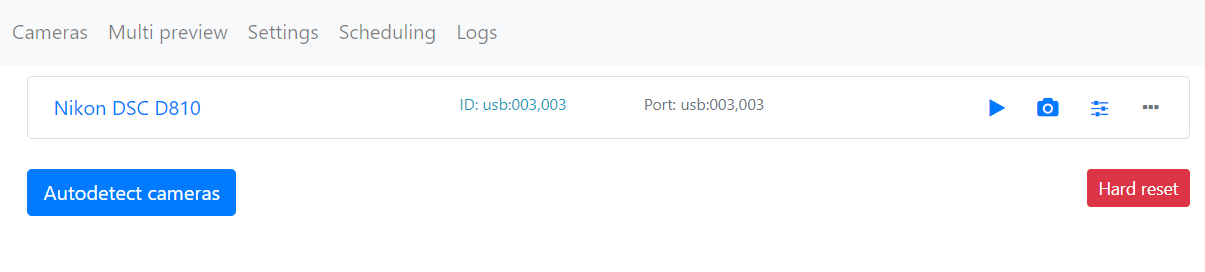
\includegraphics[width=17cm]{test-and-doc/main-view}
   \caption{Application's main page}\label{app-main-view}
\end{figure}

In the \mbox{Figure \ref{app-main-view}} it is represented the first screen the user sees. On the application start-up, the system automatically auto-detects all the cameras, so the user should see a list of the detected cameras. Each listing comes with its own set of buttons, like live preview, image capture, camera settings and camera reconnect. It also displays its Name, ID and the connected port. From this page, the user can re-detect the cameras or hard reset the ports. The hard resetting logic works by triggering the Ykush board if available. This board would then reset the USB ports which effectively re-plugs the USB ports.

\vspace{0.3cm}
\begin{figure}[!ht]
   \centering
   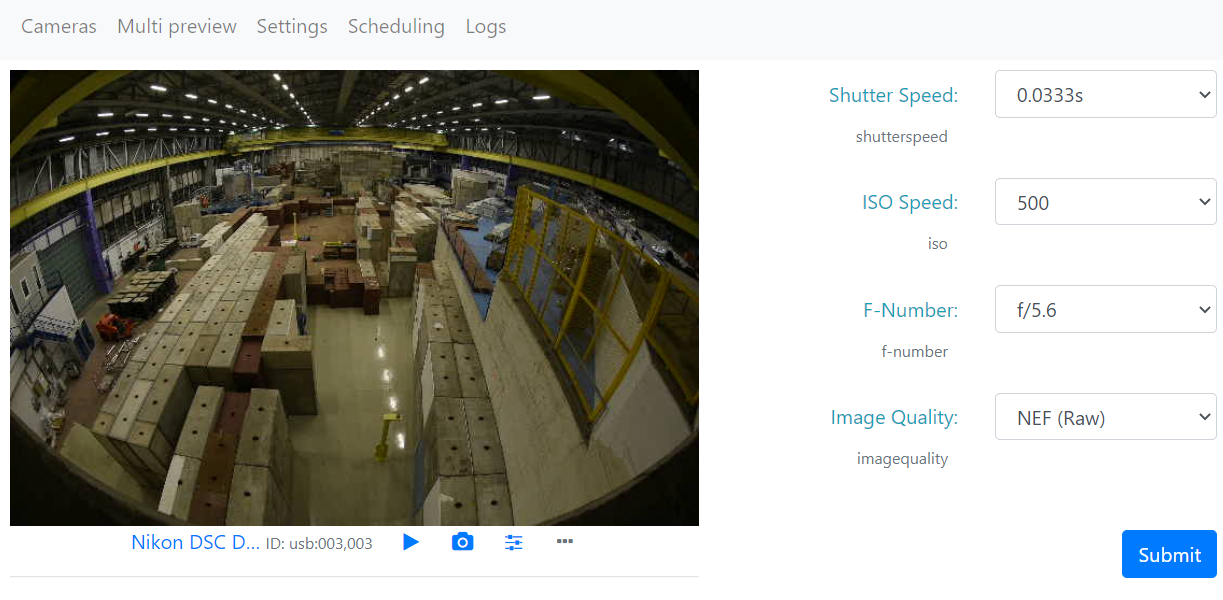
\includegraphics[width=17cm]{test-and-doc/live-preview}
   \caption{Camera live preview}\label{live-preview}
\end{figure}


\mbox{Figure \ref{live-preview}} shows the page containing the live preview of a camera. On the right side is a list with all the favorite settings. These are settings which the user may choose to display on the live preview page.

\vspace{0.3cm}
\begin{figure}[!ht]
   \centering
   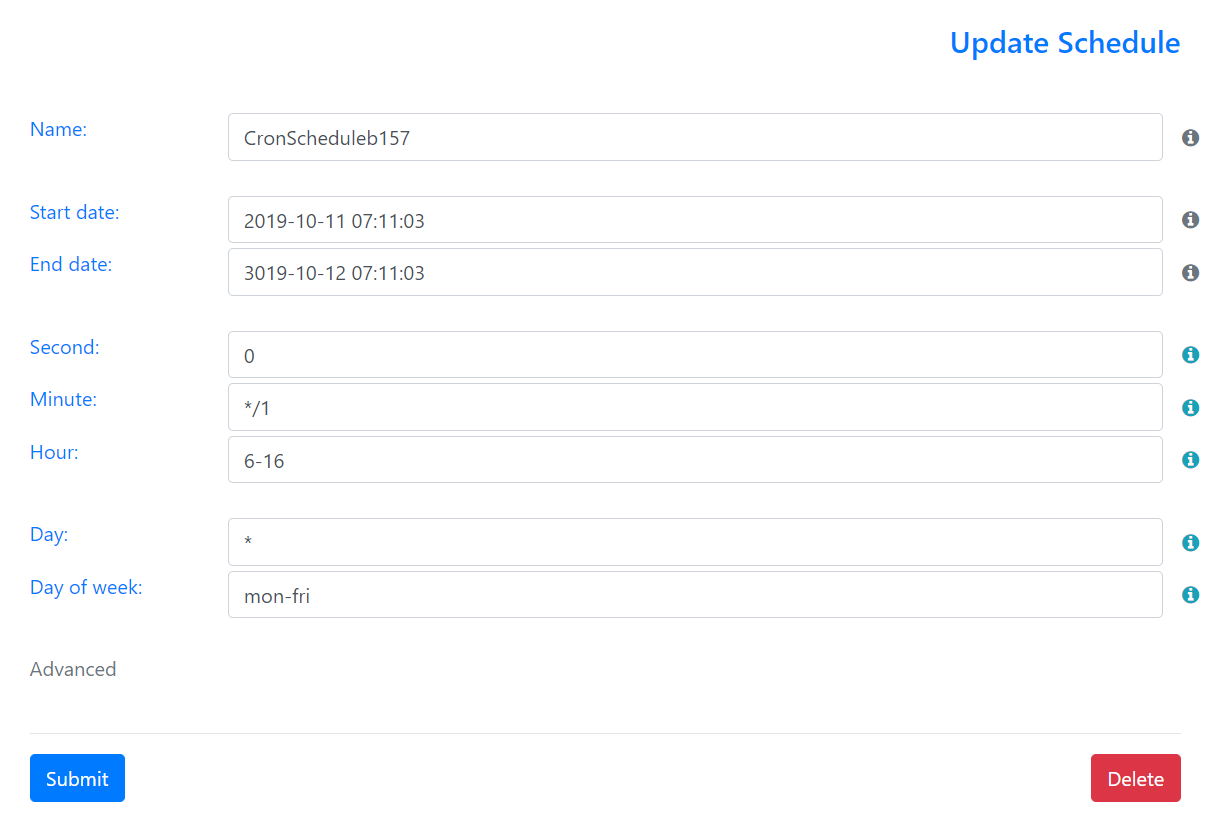
\includegraphics[width=16cm]{test-and-doc/cron-scheduling}
   \caption{Cron scheduling}\label{cron-scheduling}
\end{figure}

In the \mbox{Figure \ref{cron-scheduling}} it is represented the page where the user can configure a schedule. It's not seen in this figure, but below the Submit and Delete buttons the user can find documentation on how to correctly create or modify a schedule.

\vspace{0.3cm}
\begin{figure}[!ht]
   \centering
   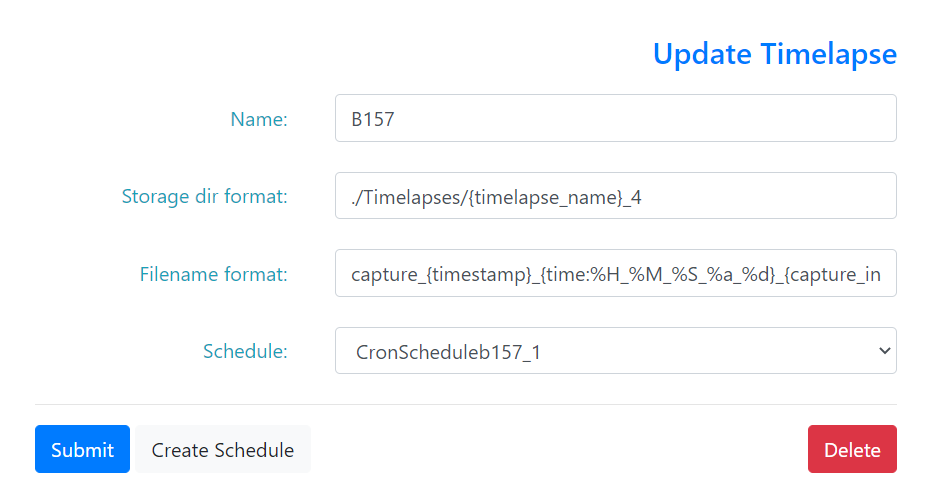
\includegraphics[width=16cm]{test-and-doc/timelapse-scheduling}
   \caption{Time-lapse scheduling}\label{timelapse-scheduling}
\end{figure}

In the \mbox{Figure \ref{timelapse-scheduling}} it is represented the page for Time-lapse configuration. The user can choose the storage directory format and the filename format. Not included in this figure, but if the user scrolls down, he would find some documentation on how to use these features. In this figure for example, the user chose to store the time-lapse photos with a filename that will contain the timestamp, the current time (in the specified format) and capture index. This format produces images in the following form:

\begin{center}
   \verb|B157_4/capture_1591376340024355_16_59_00_Fri_05_94639.nef|
\end{center}

\vspace{0.3cm}
\begin{figure}[!ht]
   \centering
   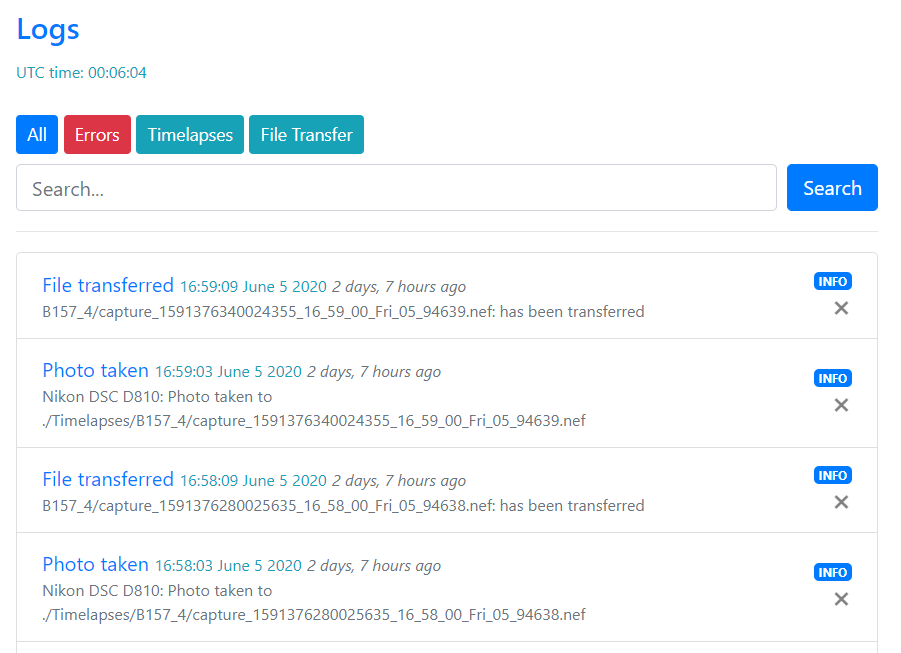
\includegraphics[width=16cm]{test-and-doc/logs}
   \caption{Logs stream}\label{logs}
\end{figure}

In the \mbox{Figure \ref{logs}} it is represented the page containing the stream of logs. Here the user can search and filter specific logs. For example he may choose to display all the errors (which is usually the case). This allows the user to see the progress of how the application is doing.

\vspace{0.3cm}
\begin{figure}[!ht]
   \centering
   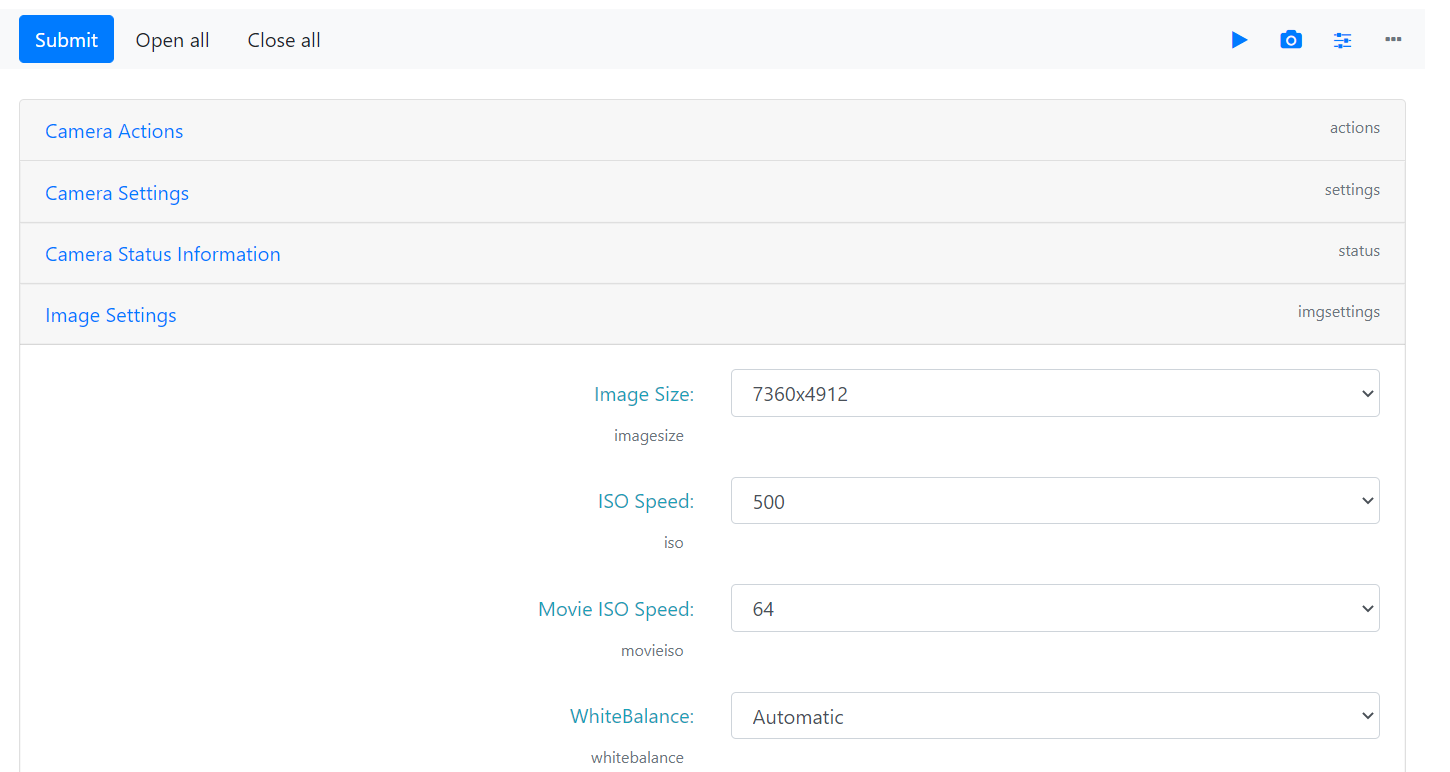
\includegraphics[width=16cm]{test-and-doc/camera-settings}
   \caption{Camera settings}\label{camera-settings}
\end{figure}

And finally, in the \mbox{Figure \ref{camera-settings}} the user can configure any of the available settings. Since \textit{gPhoto} works on a large variety of camera models, some of the displayed fields may be only read-only, that's why when a setting fails to change, an alert next to that setting appears.
